\documentclass[14pt]{extarticle}

\begin{document}
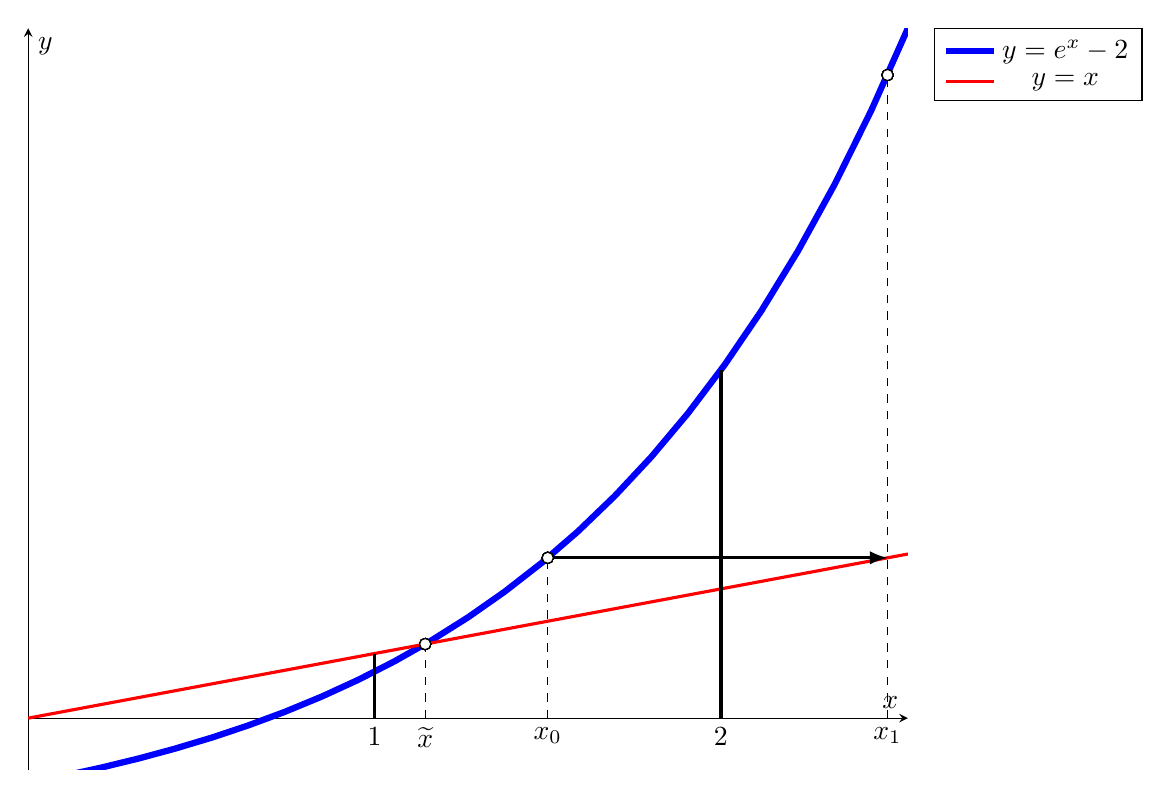
\begin{tikzpicture} [
	declare function= {
		u(\x) = e^\x-2;
		i(\x) = \x;
	},]
	\begin{axis} [
		height=11cm,
		xlabel = {$x$},
		ylabel = {$y$},
		axis x line = middle,
		axis y line = middle,
		ymin = -0.8,
		domain = 0:2.54,
		ticks = none,
		legend pos = outer north east ]

		\newcommand*{\varA}{1}
		\newcommand*{\varB}{2}
		\newcommand*{\trueX}{1.1462}
		\pgfmathsetmacro{\fa}{max(u(\varA), i(\varA))}
		\pgfmathsetmacro{\fb}{max(u(\varB), i(\varB))}
		\pgfmathsetmacro{\Xzeroth}{(\varA+\varB)/2}
		\pgfmathsetmacro{\Xfirst}{u(\Xzeroth)}
		\pgfmathsetmacro{\Xsecond}{u(\Xfirst)}

		\addplot[color=blue, line width=.08cm]{u(x)};
		\addplot[color=red, line width=.04cm]{i(x)};

		\coordinate(A) at 	(\varA,		\fa);
		\node[below](Ap) at	(\varA,		0) {$\varA$};
		\coordinate(B) at 	(\varB,		\fb);
		\node[below](Bp) at	(\varB,		0) {$\varB$};
		\coordinate(X) at 	(\trueX,	\trueX);
		\node[below](Xp) at	(\trueX,	0)
			{$\widetilde{x}$};
		\coordinate(X0) at 	(\Xzeroth,	\Xfirst);
		\node[below](X0p) at	(\Xzeroth,	0) {$x_0$};
		\coordinate(X0med) at 	(\Xfirst,	\Xfirst);
		\coordinate(X1) at 	(\Xfirst,	\Xsecond);
		\node[below](X1p) at	(\Xfirst,	0) {$x_1$};

		\addplot[mark=*,only marks, fill=white] (\trueX,\trueX)
			node[above, pos=1]{};
		\addplot[mark=*,only marks, fill=white] (\Xzeroth,\Xfirst)
			node[above, pos=1]{};
		\addplot[mark=*,only marks, fill=white] (\Xfirst,\Xsecond)
			node[above, pos=1]{};

		\draw[very thick] (Ap) -- (A)	(Bp) -- (B);
		\draw[dashed]	(Xp) -- (X)	(X0p) -- (X0)
			(X1p) -- (X1);

		\draw[-latex, very thick] (X0) -- (X0med);

		\addlegendentry{$y=e^x-2$};
		\addlegendentry{$y=x$};
	\end{axis}
\end{tikzpicture}
\end{document}
